\section {Organisation des données}

Le cas d'utilisation organisation des données constitue la troisième étape de la méthode GTD. Elle à pour but d'organiser les tâches suivant différents paramètres : \\
\begin{itemize}
\item Le contexte de l'utilisateur
\item La priorité des tâches
\item Le temps disponible pour les tâches
\item L'énergie disponible à la réalisation des tâches
\end{itemize}


\subsection*{Cockburn de l' organisation des données}


\begin{center}
\begin{tabular}{|p{1.1in}|p{0.6in}|p{2in}|p{2.0in}|} \hline 
\textbf{Cas d'utilisation }& \multicolumn{3}{|p{3.2in}|}{Organiser les données} \\ \hline 
\textbf{Acteur} & \multicolumn{3}{|p{3.2in}|}{Utilisateur} \\ \hline 
\textbf{Parties 
prenantes et intérêts }& \multicolumn{3}{|p{5in}|}{A partir des taches existantes 
(qui résulte du traitement des données), on les organise au sein d'un projet 
et par rapport à un contexte donné} \\ \hline 
\textbf{Niveau} & \multicolumn{3}{|p{3.2in}|}{Utilisateur} \\ \hline 
\textbf{Portée} & \multicolumn{3}{|p{3.2in}|}{Système GTD} \\ \hline 
\textbf{Pré-conditions} & \multicolumn{3}{|p{5in}|}{On dispose d''une liste de taches résultants 
de l'étape traitement des données.} \\ \hline 
\textbf{Post-conditions} & \multicolumn{3}{|p{5in}|}{Les taches sont organisées au sein 
de projets} \\ \hline 
\textbf{Scénario nominal} & \textbf{Etapes}  & \multicolumn{2}{|p{2.5in}|}{\textbf{Action}} \\ \hline 
~ & 1 & \multicolumn{2}{|p{4in}|}{Identification des tâches qui contribuent à la 
réalisation d'un même travail.} \\ \hline 
~ & 2 & \multicolumn{2}{|p{4in}|}{Regroupement des taches au niveau de projets} \\ \hline 
~ & 3 & \multicolumn{2}{|p{4in}|}{Les 
tâches sont organisées en fonction du contexte, du temps disponible, de la capacité 
physique (énergie) et de la priorité} \\ \hline 
~ & ~ & \multicolumn{2}{|p{2.5in}|}{~} \\ \hline 
~ & ~ & \multicolumn{2}{|p{2.5in}|}{~} \\ \hline 
\textbf{Extensions} & \textbf{Etapes} & \textbf{Condition} & \textbf{Action} \\ \hline 
~ & 2.a & Une tâche est à réaliser sans dépendances & On ne créer pas de projet pour 
celle-ci. \\ \hline 
~ & 3.a & Une~tâche ne peut pas être réalisée à un instant (t), compte tenu du contexte & On 
lui attribue une période de réalisation appropriée pour son contexte \\ \hline 
\textbf{Priorité} & \multicolumn{3}{|p{3.2in}|}{Très élevée (5/5)} \\ \hline 
\textbf{Performance} & \multicolumn{3}{|p{3.2in}|}{~} \\ \hline 
\textbf{Fréquences} & \multicolumn{3}{|p{5in}|}{De façon obligatoire après chaque traitement 
d'information.~} \\ \hline 
\end{tabular}\end{center}


Comme on peut le voir l'organisation se divise en deux grandes étapes :\\
\begin{itemize}
\item Le regroupement des tâches participant à un même travail
\item L'organisation des tâches en fonction de leurs contextes, des priorités.
\end{itemize}


\subsection*{Diagramme d'objets de l' organisation des données}

\subsubsection{Vision du système avant l'étape d'oganisation}
Sur le diagramme suivant, les tâches ne sont pas reliées entre elles. Elles sont indépendantes et disposent d'un état et d'un contexte. L'espace de travail est également lié à un contexte, cette relation n'a cependant pas la même signification que pour une tâche : en effet, le contexte par défaut d'un projet regroupe les propriétés que devront (au moins) posséder les tâches affectées à ce même projet. L'exemple présenté ci-dessous illustre parfaitement le fait qu'un espace de travail regroupe des tâches de contextes différents.

\begin{figure}[H]
\begin{center}
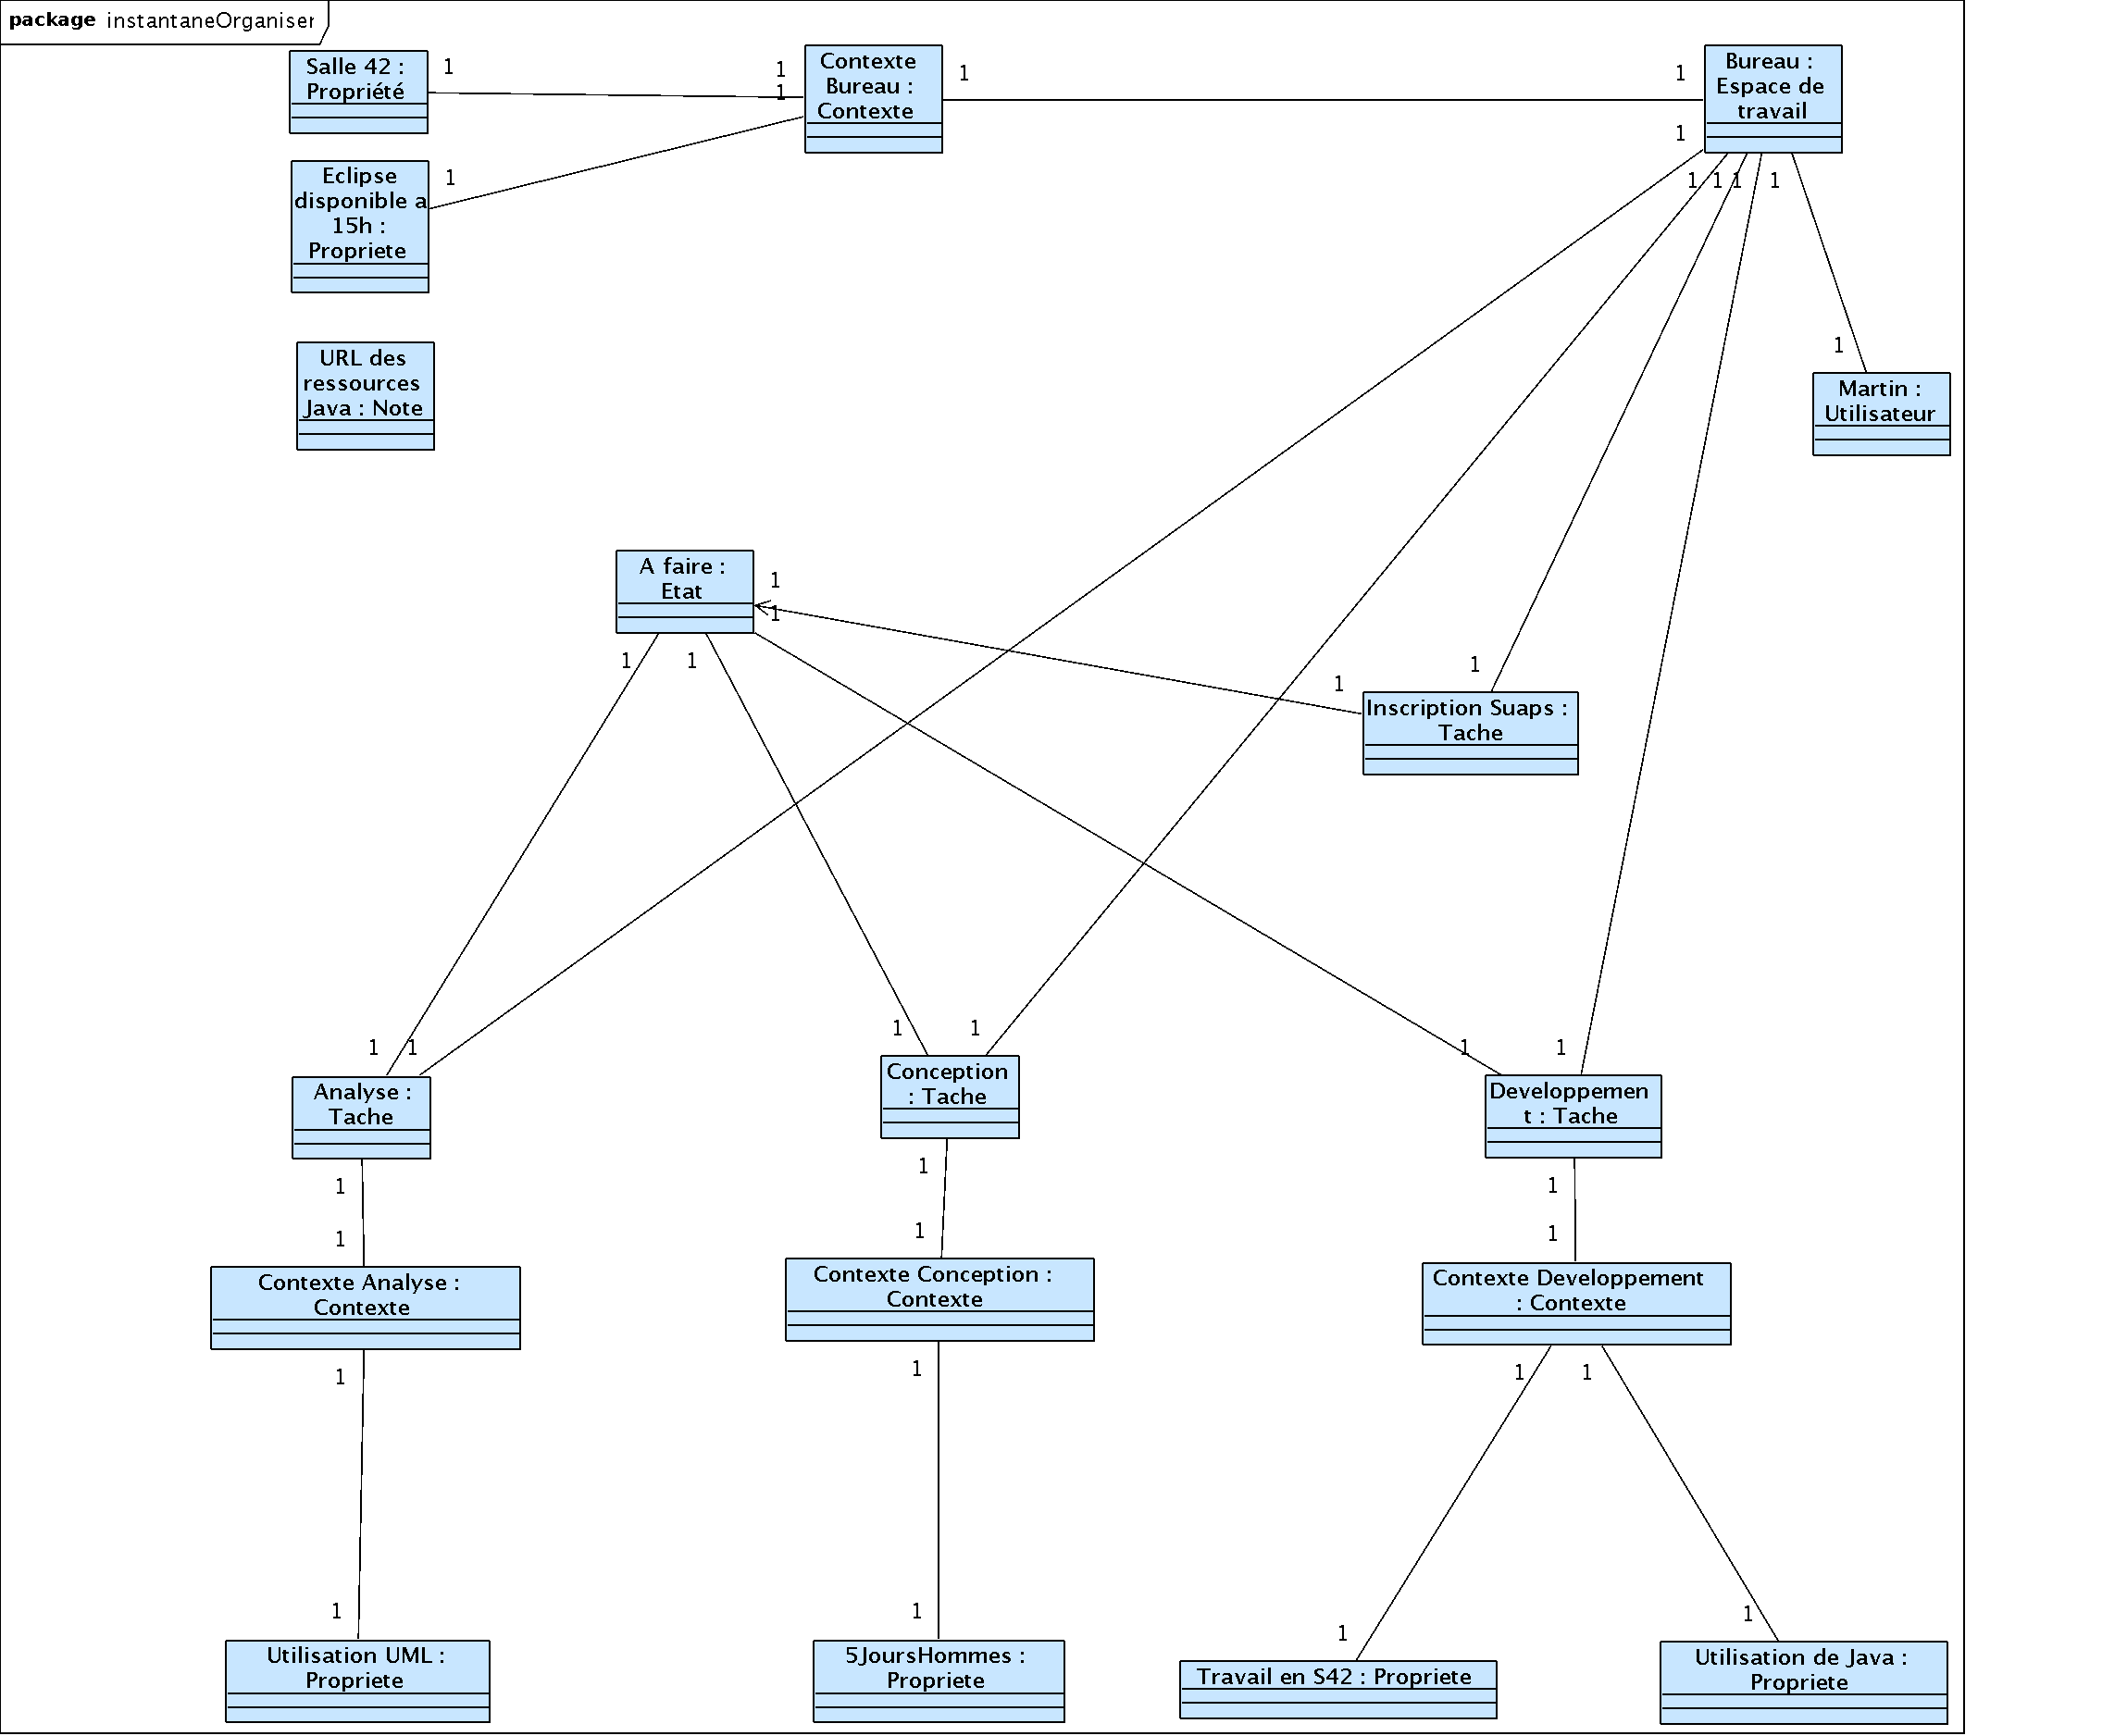
\includegraphics[scale=0.35,angle=90]{diagrams/instantaneOrganiserBefore.png}
\caption{Diagramme UML Objet - Instantanné avant l'étape organisation}
\end{center}
\end{figure}


\subsubsection{Vision du système après l'étape d'oganisation}
Sur le schéma suivant, une étape d'organisation à été effectuée. Ainsi, les tâches sont donc reliées entre elles grâce à la relation \textit{tâche précédente}. De plus, certaines tâches correspondent à la réalisation d'un même travail. C'est pourquoi elles sont contenues dans un projet, ici Projet GLO. On observe également que par rapport au schéma précédent, les tâches sont reliées à l'espace de travail à travers un objet vue. La vue \textit{Agenda} ordonne les tâches selon des critères de temps, se limitant aux tâches courantes et enfin selon le contexte actuel : En effet, dans toutes les \textit{Vues} comme \textit{Agenda} ou \textit{Echéancier}, le contexte courant (au moment où la demande est faite) est un critère de sélection des tâches à ordonner dans des \textit{Vues} . Ici par exemple, le contexte de la tâche \textit{inscription suaps} ne correspond pas au contexte définit dans la vue, c'est pourquoi la tâche n'est pas associée à cette vue.

\begin{figure}[H]
\begin{center}
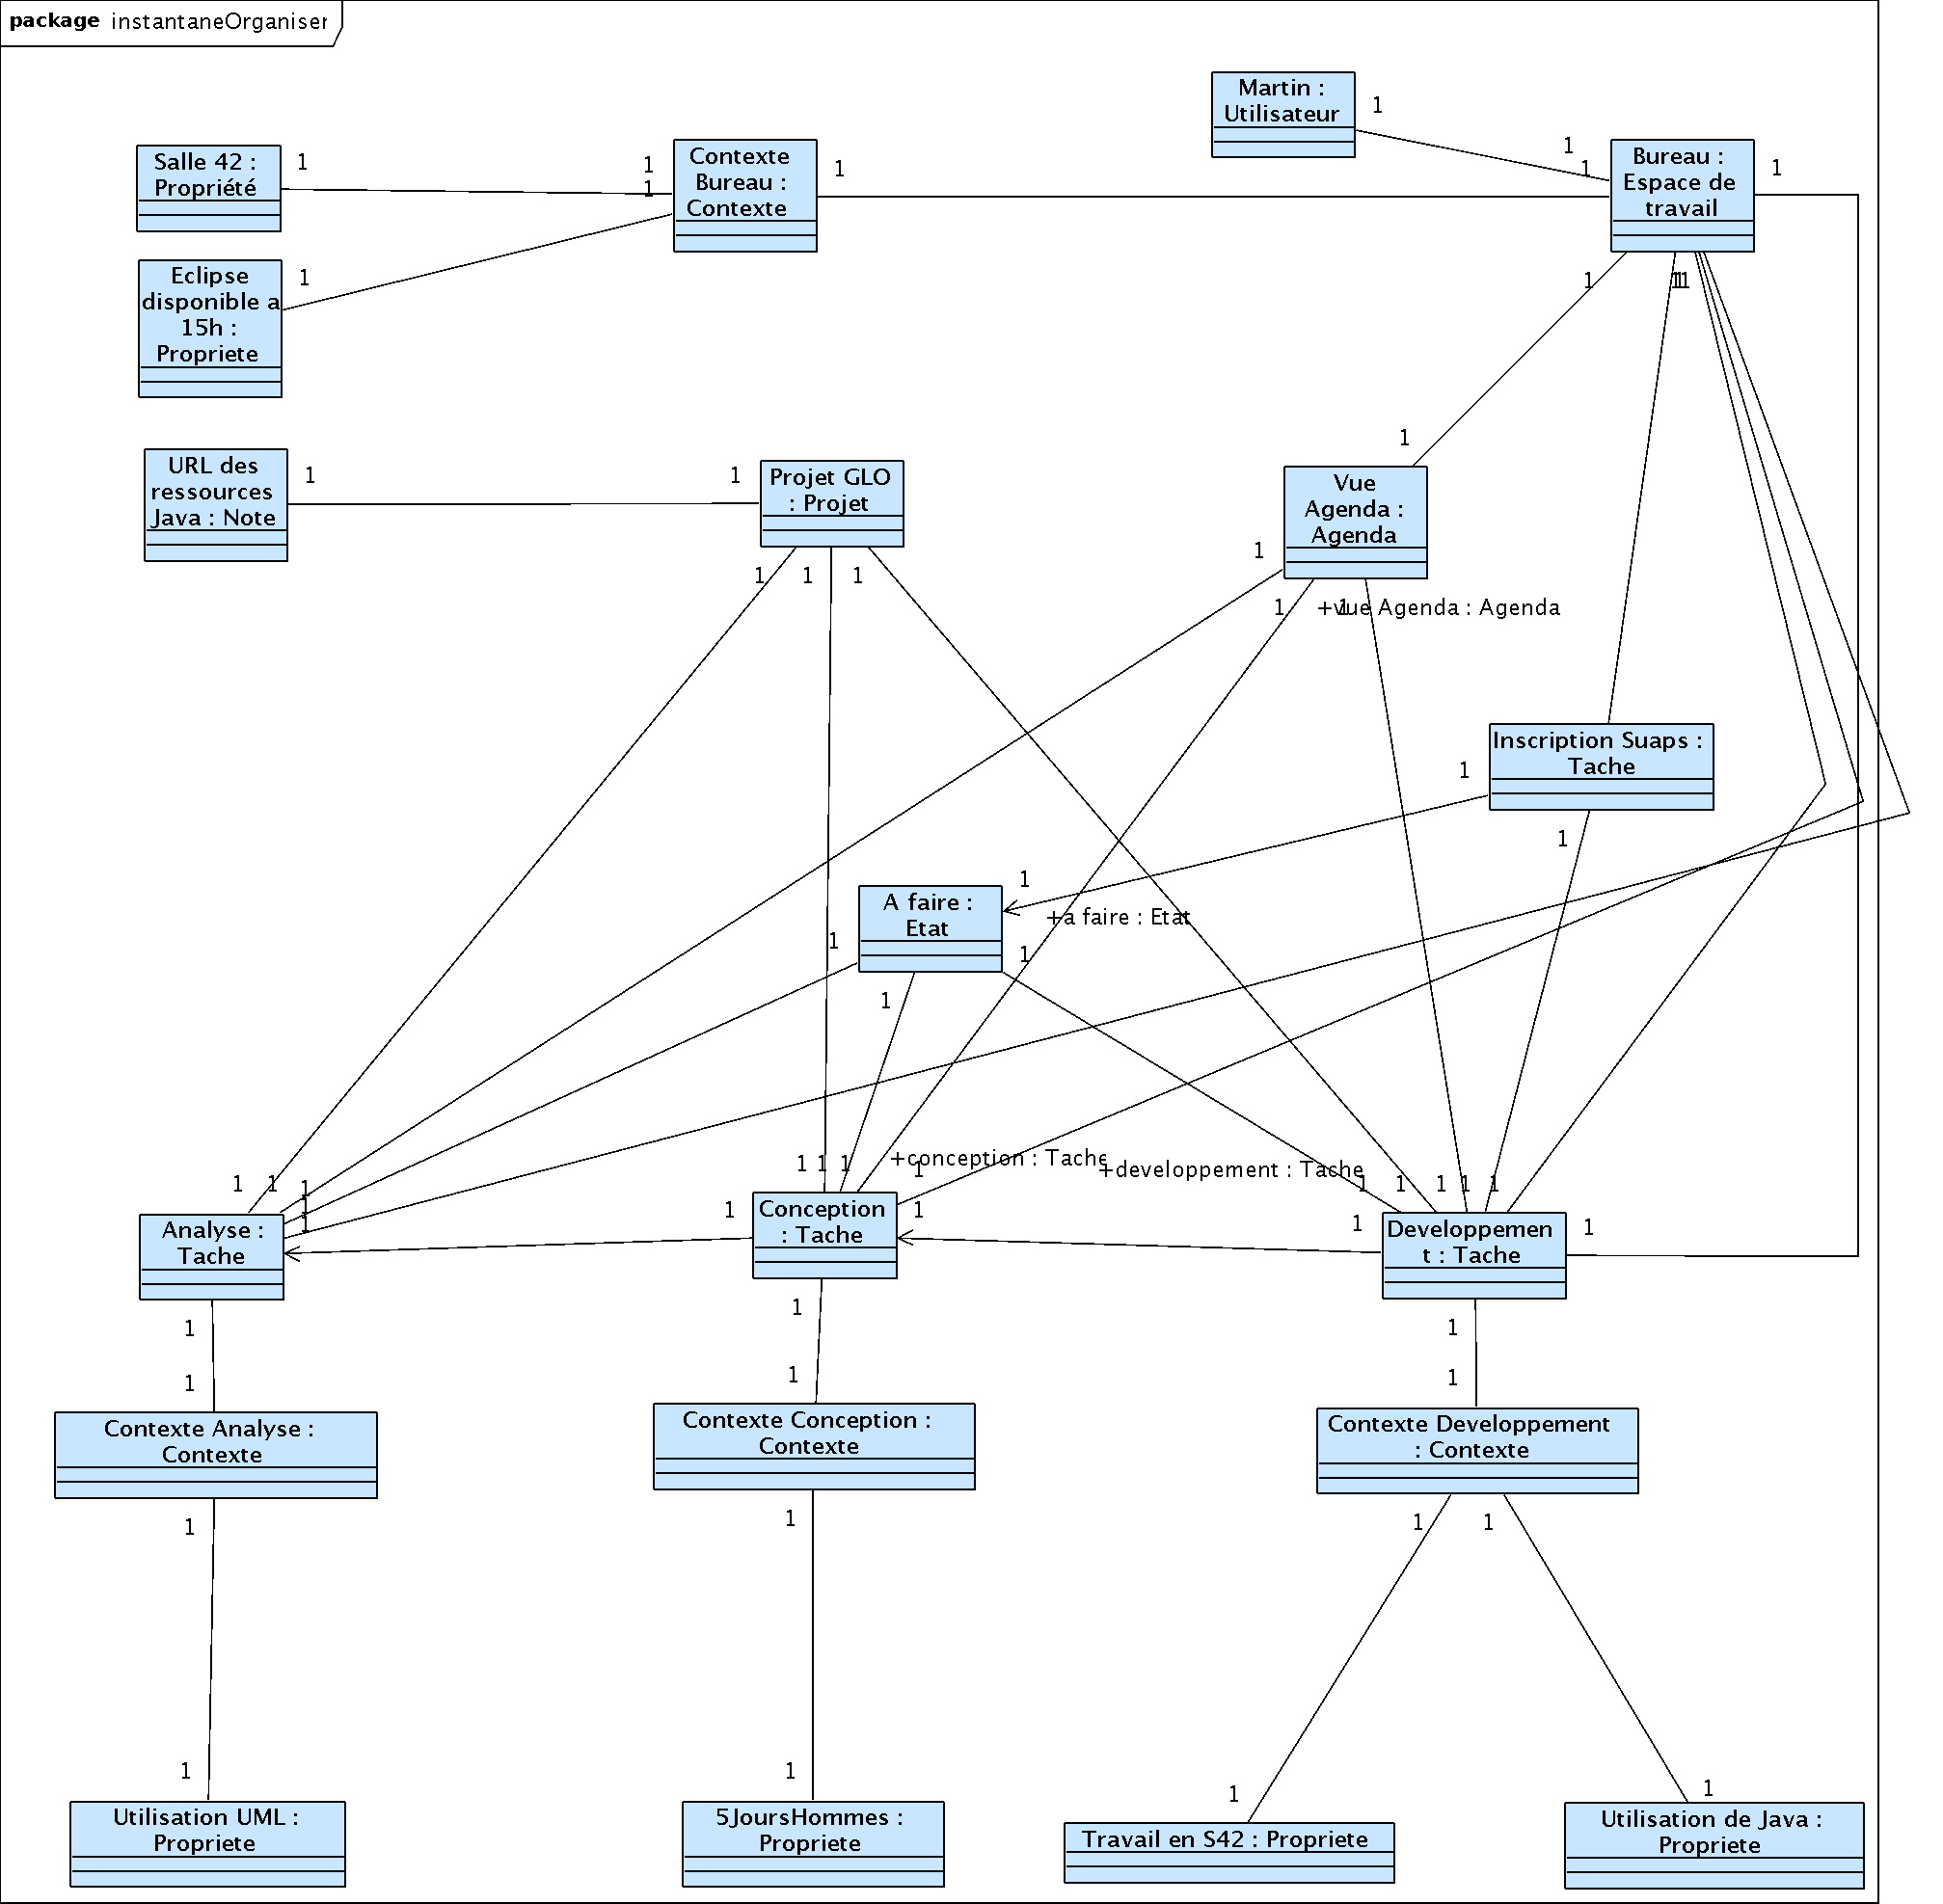
\includegraphics[scale=0.29,angle=90]{diagrams/instantaneOrganiserAfter.png}
\caption{Diagramme UML Objet - Instantanné après l'étape organisation}
\end{center}
\end{figure}

